\documentclass[10pt,a4paper,twocolumn]{article}
\usepackage[T1]{fontenc}
\usepackage[utf8]{inputenc}
\usepackage{anysize, longtable}
\usepackage{amsthm, amsfonts, amsmath, amssymb, booktabs, float}
\usepackage{sectsty, csquotes, xcolor, xspace, setspace, listings}
\usepackage{graphicx, tabularx, changepage, multirow, subcaption}
\usepackage{algorithm, algpseudocode, multicol, cuted, colortbl}
\usepackage{makecell, supertabular, xpatch}
\usepackage[hidelinks,bookmarksdepth=3]{hyperref}
\usepackage[capitalise]{cleveref}
\usepackage[inline]{enumitem}
\usepackage[english]{babel}
\usepackage{microtype}
\usepackage{libertinus}
\usepackage[scale = 0.85]{plex-mono}
\usepackage[maxbibnames=99,maxcitenames=1,style=authoryear]{biblatex}
\usepackage[moderate,mathdisplays=normal]{savetrees}
\usepackage{titlesec}
\usepackage{tikz}

\usetikzlibrary{fit, shapes.geometric, shapes.symbols, positioning, shapes.misc, calc, arrows.meta, patterns, backgrounds, decorations, decorations.markings, decorations.pathreplacing, shadows, hobby, decorations.pathmorphing}

\xpatchbibmacro{cite}
 {\printnames{labelname}}
 {\printtext[bibhyperref]{\printnames{labelname}}}
 {}{}

\xpatchbibmacro{textcite}
 {\printnames{labelname}}
 {\printtext[bibhyperref]{\printnames{labelname}}}
 {}{}

\makeatletter

\theoremstyle{plain}
\newtheorem{theorem}{Theorem}
\newtheorem{lemma}{Lemma}

\theoremstyle{definition}
\newtheorem{definition}{Definition}
\newtheorem{example}{Example}

\theoremstyle{remark}
\newtheorem*{note}{Note}
\newtheorem*{remark}{Remark}

\newcommand{\inlinecode}[1]{\lstinline[basicstyle=\ttfamily,columns=fixed]$#1$}
\lstset{basicstyle=\setstretch{0}\small\ttfamily,breaklines=true,columns=fixed,captionpos=b,xleftmargin=0.5cm}

\newlength{\offsetpage}
\newenvironment{widepage}[1][2cm]{
  \setlength{\offsetpage}{#1}
  \begin{adjustwidth}{-\offsetpage}{-\offsetpage}
  \addtolength{\linewidth}{2\offsetpage}
}{\end{adjustwidth}}

\algnewcommand{\IIf}[1]{\State \algorithmicif\ #1\ \algorithmicthen}
\algnewcommand{\IElse}[1]{\algorithmicelse\ #1}
\algnewcommand{\EndIIf}{\unskip\ \algorithmicend\ \algorithmicif}

\addbibresource{biblio.bib}

\allowdisplaybreaks
\marginsize{2.0cm}{2.0cm}{1.25cm}{1.25cm}
\setcounter{tocdepth}{2}
\setlist[itemize]{topsep=0pt, partopsep=0pt, parsep=0pt, itemsep=\parskip}
\setlist[enumerate]{topsep=0pt, partopsep=0pt, parsep=0pt, itemsep=\parskip}
\titlespacing*{\paragraph}{0pt}{0.5\baselineskip}{0.5\baselineskip}
\captionsetup[figure]{aboveskip=5pt}
\captionsetup[subfigure]{aboveskip=3pt}

\title{Markerless 3D Human Pose Tracking}
\author{Roland Bernard, 19598, \inlinecode{rolbernard@unibz.it}}
\date{September 2026}

\def\maketitle{
\begin{strip}
  \begin{adjustwidth}{5mm}{5mm}
    \vspace{-4.5em}
    \noindent{\small\bfseries Project Report -- Capstone Project 2025/2026\par}
    \vskip 0.25em
    \noindent{\LARGE\bfseries \@title\par}
    \vskip 1em
    \noindent{\large \@author\par}
    \vskip 1em
    \noindent{{\scriptsize Tutor} Oswald Lanz \quad \quad {\scriptsize Domain Expert} Marco Boschetti (Covision Lab)\par}
    \vskip 0.5em
    \noindent{\hspace{0.12mm} {\scriptsize Date} \@date\par}
    \vskip 1em
  \end{adjustwidth}
\end{strip}
}
\renewenvironment{abstract}{
  \vskip 1em
  \begin{quote}
  {\normalsize \abstractname\par}
  \small
}{
  \end{quote}
  \vskip 1em
}

\makeatother

\input{tikzfigures/defs.tex}

\begin{document}

\maketitle

\begin{abstract}
The tracking of 3D human poses represents a crucial area in computer vision, with widespread applications across robotics, automated surveillance, healthcare, and entertainment. This project explores a tracking-by-detection framework designed to fuse multi-view 2D pose estimations from synchronized camera feeds into coherent, temporally consistent 3D skeletal trajectories. A system utilizing the YOLO26-pose model family for 2D keypoint extraction and extended Kalman filtering for 3D state estimation is developed, implemented, and evaluated. The project further explores the inclusion of skeletal constraints and a custom YOLO head to increase performance.

The resulting system was evaluated on eight video sequences from the CMU Panoptic dataset, benchmarking the impact of different system configurations on task performance and computational efficiency. Computational runtime analysis shows that the 2D detection phase dominates the processing, consuming between 67\% and 93\% of per-frame execution time and scaling linearly with the number of camera feeds. Furthermore, increasing the viewpoint density improves tracking and 3D reconstruction precision. For the smallest model configuration, scaling from 4 to 16 cameras reduces the Mean Per-Joint Position Error (MPJPE) from 8.25 cm down to 3.83 cm while also improving Multi-Object Tracking Accuracy (MOTA) from 0.78 to 0.93. The inclusion of skeletal constraints and tuning of the different components using the dataset also improves performance, with a 4 camera setup improving from a MOTA of 0.78 with the baseline to 0.90 for the fully tuned model. MPJPE also improves from 8.25 cm to 4.92 cm in the same setting.
\end{abstract}


\section{Introduction} \label{into}

This capstone project focuses on markerless 3D human pose tracking. The estimation and tracking of 3D human poses is an important research area in computer vision, driven by its broad range of immediate applications across multiple domains. For example, in robotics and human-robot interactions it can find application in industrial environments and collaborative workspaces where robots must accurately perceive human poses and predict movements to maintain safe operational boundaries and avoid collisions with dangerous machinery \parencite{svenstrup2009pose,dondrup2015real,koppula2015anticipating}. Similarly, for crowd control tracking of multi-person trajectories in public spaces facilitates anomalous behavior detection, crowd density planning, and automated surveillance \parencite{sultani2018real,luo2021multiple}. Other impactful applications can be found in healthcare, such as gait analysis, automated fall detection, and remote patient monitoring \parencite{han2025comprehensive,gaya2024deep}. Finally, human pose estimation and tracking can find applications also in the entertainment domain, such as the use of real-time motion capture for virtual avatars or natural body-based control interfaces for gaming \parencite{mehta2020xnect}.

Despite the maturity of real-time 2D human pose estimation, transferring these methods to a robust and real-time capable 3D setting remains a challenging task due to issues such as depth ambiguities, severe self-occlusions, and the high perspective variance of human motion \parencite{zheng2023deep,nogueira2025markerless}. The primary objective of this project is to design, implement, and evaluate a computer vision architecture capable of tracking the skeletal movement of multiple people from 2D pose estimations extracted from multiple views by 2D human pose estimation models. The system should be able to fuse the information gained from the 2D video frames of multiple camera viewpoints into coherent and temporally consistent 3D pose trajectories.

For the evaluation of the result, this project will use a subset of the CMU Panoptic dataset \parencite{Joo_2015_ICCV,Joo_2017_TPAMI}, which contains videos captured from multiple calibrated cameras together with ground truth pose and tracking information for each frame. Using this evaluation set this project further aims to investigate the impact of model capacity as well as the viewpoint count on both the achieved tracking accuracy and the runtime efficiency of the system. For qualitative analysis the project also makes use of the SALSA dataset \parencite{alameda2015salsa}. This dataset does not contain ground truth pose annotations, but represents a more difficult application scenario.

The remainder of this report is structured as follows: \Cref{background} reviews the relevant theoretical background underlying the project. \Cref{methodology} gives an overview of the developed tracking system as well as detailed explanations of each component. \Cref{experiments} describes the used dataset and the evaluation strategy including evaluation metrics. \Cref{results} presents the quantitative and qualitative evaluation results. Finally, \Cref{conclusion} concludes the report with a summary of the findings and outlines limitations, highlighting potential areas for further improvements.



\section{Background} \label{background}

This section of the report covers relevant background knowledge necessary to understand the developed pose tracking system. A high level overview of a number of computer vision related topics is given.


\subsection{Object Detection and Pose Estimation} \label{detection}

In object detection the goal is to localize all object, the number of which is not known a priori, in images \parencite{Lanz2026Notes}. Like many computer vision recognition tasks, the field of object detection has evolved significantly with the introduction of deep learning \parencite{Lanz2026Notes}. Deep learning-based object detection has evolved through two primary paradigms. Anchor-based models, such as R-CNN or YOLO, rely on predefined bounding box priors of various scales and predicting offsets from these anchors. In contrast, anchor-free models predict bounding boxes directly from point features or keypoint combinations.

In two stage detector models such as R-CNN, there are two separate inference stages \parencite{bharati2019deep}. The first stage generates a large number of candidate regions and the second stage then classifies these regions. Fast R-CNN \parencite{girshick2015fast} and Faster R-CNN \parencite{ren2015faster} improve inference speed over the original R-CNN by using a shared feature backbone for both stages and by using a Region Proposal Network to create candidate regions.

In contrast to these two-stage detectors, the YOLO model used in this project is a single stage detector \parencite{jiang2022review}. It works by dividing the input image into multiple grids of different resolutions. Then a CNN based architecture is employed to extract features for each of the grid positions. Finally, one or more prediction head are applied to the resulting feature maps to simultaneously predict both object presence and bound box offsets from grid location defined anchors. The main advantage of single-stage approaches is that they are usually faster than two-stage approaches, although they often perform worse in practice \parencite{Lanz2026Notes}.

Once an object is detected, one can append extra heads to the feature maps to also predict other properties about the objects. An example of this approach is the Mask R-CNN architecture \parencite{he2017mask}, which predicts instance masks for each detected object \parencite{Lanz2026Notes}. However, this approach can also be applied to Human Pose Estimation, where the additional output head of the network is instead used to predict keypoint locations \parencite{maji2022yolo}. This approach is taken by the YOLO26 models used in this project \parencite{ultralyticsYOLO,sapkota2025yolo26,sapkota2025ultralytics}. Furthermore, as part of this work an additional custom head is trained for the YOLO26 model as explained in \cref{yolo-head}.


\subsection{Object Tracking} \label{tracking}

Detecting objects or estimating poses in individual frames is insufficient for many applications \parencite{Lanz2026Notes}. Instead, what is often required is to associate detections with the physical objects they belong to and model how those evolve over time. This problem is called object tracking. The approach taken in this project is tracking-by-detection. This method can be divided into three essential steps, detection, association, and filtering. In detection, candidate objects are detected in individual frames. Then, these detections are assigned to concrete objects in the association step. Finally, filtering is used to determine the most probable state of the object given the associated detections. Filtering is responsible for refining the noise inherently present in the detection using probabilistic models and preceding observations. This subsection will focus on the association and filtering steps, while the detection step has already been discussed in \cref{detection},

In many application multiple targets must be tracked at the same time. To understand which detection belongs to which underlying object, association must be performed \parencite{Lanz2026Notes}. A typical way to proceed it to predict object from the previous frame and to use those predictions to associate detections to the objects. This association can be performed using an association measure, which is a measure indicating the distance or similarity between a predicted object track and a detection. A naive approach, and also the one applied in this project, is to measure the overlap of the prediction and the detection \parencite{bewley2016simple}. Alternative approaches can include color histograms or optical flow and measure agreement \parencite{Lanz2026Notes}. It is also possible to used metric learning, where a deep learning model is used to extract features for computing the association measure.

After an association measure has been established, it is still necessary to actually perform the association \parencite{Lanz2026Notes}. A naive approach can be to consider all detections within some gating area of the prediction and then associate the closest of these detections to the prediction. The distance in this context can also consider the probabilistic model of the prediction to find most probable detections. However, this nearest neighbor approach can easily fail due to ambiguities. A better approach is to use a bipartite graph matching based framework. In this framework, the problem is modeled as a bipartite graph from predictions to detections, with edges weighted by the association metric. This can be formulated as the following integer linear programming problem:
\begin{align*}
  & \operatorname*{argmax}_{\mathbf{Z}} \sum_{i=1}^{M} \sum_{j=1}^{N} s_{ij} z_{ij} \\
  & s.t. \quad \forall j: \sum_{i=1}^{M} z_{ij} = 1 \quad \forall i: \sum_{j=1}^{N} z_{ij} = 1 \quad z_{ij} \in \{0, 1\}
\end{align*}
where $s_{ij}$ and $z_{ij}$ are respectively the association metric and association between prediction $i$ and detection $j$. This problem can then be solved either using a greedy algorithm, or as has been done for this project, using globally optimal algorithms such as the Hungarian method \parencite{kuhn1955hungarian}. Finally, another possible approach to association is to used advanced graph-based deep learning networks.

After detections and objects have been associated, it is necessary to perform the filtering step \parencite{Lanz2026Notes}. It is crucial to understand that detections differ from the underlying state that we try to understand. Aside from being noisy, detections might also be missing some information of interest in the object. For example, object detections usually do not include velocity, and still we would like to infer it from the detections. When represented as using a Markov model, the state of a target at any given time step depends only on that targets state in the previous time step. Further, the observation or detection at any time step depends only on the targets current state. One way to evaluate this process is using recursive Bayesian estimation, also called Bayesian filtering.

Bayesian filtering is applied in two phases. First, the prediction step is used to model the target states distribution using only the past observations. Due to the conditional independence assumption of the hidden Markov model, this probability distribution of the hidden state can be computed as followed:
\begin{align*}
  p(\mathbf{x}_t|\mathbf{z}_{1:t-1}) &= \int p(\mathbf{x}_t, \mathbf{x}_{t-1} | \mathbf{z}_{1:t-1}) d\mathbf{x}_{t-1} \\
  &= \int p(\mathbf{x}_t | \mathbf{x}_{t-1}, \mathbf{z}_{1:t-1}) p(\mathbf{x}_{t-1} | \mathbf{z}_{1:t-1}) d\mathbf{x}_{t-1} \\
  &= \int p(\mathbf{x}_t | \mathbf{x}_{t-1}) p(\mathbf{x}_{t-1} | \mathbf{z}_{1:t-1}) d\mathbf{x}_{t-1}
\end{align*}
where $p(\mathbf{x}_t | \mathbf{x}_{t-1})$ defines out motion model, and $p(\mathbf{x}_{t-1} | \mathbf{z}_{1:t-1})$ is the posterior distribution after applying all previous observations. After prediction, we want to incorporate the information gained by the new observation. This can be achieved as follows by applying Bayes' rule:
\begin{align*}
  p(\mathbf{x}_t \mid \mathbf{z}_{1:t}) &\propto p(\mathbf{z}_t \mid \mathbf{x}_t) p(\mathbf{x}_t \mid \mathbf{z}_{1:t-1})
\end{align*}
where $p(\mathbf{z}_t \mid \mathbf{x}_t)$ models the observation process.

The equations of the Bayesian filtering algorithm can be implemented by representing the probability distributions at each time step in parametric form, such as in Kalman filtering \parencite{Lanz2026Notes,bar2001estimation}, or in nonparametric form, such as with particle filters. In a linear Kalman filter the motion and observation models are defined as:
\begin{align*}
  \mathbf{x}_t &= \mathbf{F}_t \mathbf{x}_{t-1} + \mathbf{B}_t \mathbf{u}_t + \mathbf{w}_t, \quad \mathbf{w}_t \sim \mathcal{N}(\mathbf{0}, \mathbf{Q}_t) \\
  \mathbf{z}_t &= \mathbf{H}_t\mathbf{x}_t + \mathbf{v}_t, \quad \mathbf{v}_t \sim \mathcal{N}(\mathbf{0}, \mathbf{R}_t)
\end{align*}
The optimal closed-form solution is the standard Kalman Filter, which updates the mean $\mathbf{\bar{x}}_t$ and covariance $\Sigma_t$ of $\mathbf{x}_t$ through linear projection and gain computation.

While the linear Kalman filter is applicable in cases where both the motion and observation model are linear, in our application of multi-view tracking, the measurement model is non-linear because 3D world coordinates must project onto a 2D camera plane. For this reason, this project makes use of extended Kalman filtering. We define the observation function to be $\mathbf{z}_t = h(\mathbf{x}_t) + \mathbf{v}_t$. The extended Kalman filter linearizes this non-linear function using a first-order Taylor expansion around the predicted state estimate $\mathbf{\bar{x}}_t$:
\begin{align*}
h(\mathbf{x}_t) \approx h(\mathbf{\bar{x}}_t) + \mathbf{J}_h (\mathbf{x}_t - \mathbf{\bar{x}}_t)
\end{align*}
where $\mathbf{J}_h$ is the Jacobian matrix evaluated at $\mathbf{\bar{x}}_t$. In the update step the Jacobian matrix is the used in place of the linear observation matrix $\mathbf{H}_t$ to update the covariance and calculate Kalman gain.


\subsection{Projective Geometry} \label{calibration}

The dataset used in this project already contains camera calibration parameters for all camera views. Still, understanding the meaning of these parameters and how they relate to the image formation process is critical for the correct implementation for the triangulation algorithm as well as for modeling the observation process. The mapping of 3D points to 2D pixels is defined mathematically through the pinhole camera model \parencite{Lanz2026Notes,hartley2003multiple}. Unlike a physical pinhole camera, which would invert the image, the mathematical model places the image plane in front of the focal point for convenience. The full perspective projection model linking a homogenous 3D world coordinate $\tilde{x}_w$ to a homogenous 2D sensor pixel $\tilde{x}_s$ is given by:
\begin{align*}
  \tilde{x}_s &= \mathbf{K} [\mathbf{R} | \mathbf{t}] \tilde{x}_w = \mathbf{P} \tilde{x}_w
\end{align*}
where $\mathbf{P}$ is the full $3 \times 4$ projection matrix. It decomposes into intrinsic parameters $\mathbf{K}$ and extrinsic parameters $\mathbf{R} and \mathbf{t}$. For a perspective projection, 3D points $\tilde{x}_s$ in the local camera coordinate system are mapped to the image plane by dividing them by their depth $Z$ component.

The assumption of linear projection made by the above pinhole camera model, where straight lines remain straight, is violated by physical camera lenses, introducing distortions \parencite{Lanz2026Notes}. These must be modeled to accurately project points or undistort pixel coordinates. Two types of distortions are typically modeled. First, radial distortion causes points to bend outward inward. It is modeled relative to the squared radius $r^2 = x^2 + y^2$. Second, tangential distortion arises when the lens is not perfectly parallel to the imaging sensor.


\subsection{Multi-View Triangulation} \label{triangulate}

Even once corresponding points across multiple camera views have been identified, their 3D position $\tilde{x}_w$ must still be reconstructed from the 2D pixel locations. Rays back-projected from pixels will nearly never intersect perfectly in 3D space due to measurement noise. As such, a noise robust algorithm must be used that can recover 3D coordinates using multiple noise 2D projections \parencite{Lanz2026Notes,hartley2003multiple}. If we denote $\tilde{x}_i^s$ the homogeneous 2D observation in the $i$-th camera, and $\mathbf{P}_i$ the projection matrix of that that camera, because $\tilde{x}_i^s$ and the projected point $\mathbf{P}_i \tilde{x}_w$ represent the same point up to scale, their cross product must be zero:
\begin{align*}
  \tilde{x}_i^s \times \mathbf{P}_i \tilde{x}_w &= 0 \\
\end{align*}
This cross product yields a set of three linear equations for each camera view. However, the third is a linear combination of the first two, so it can be discarded. By stacking the equations from $N \ge 2$ camera views, we obtain a homogeneous linear system $\mathbf{A} \tilde{x}_w = 0$. Because $\tilde{x}_w$ is defined only up to scale, we impose the constraint $||\tilde{x}_w|| = 1$. The optimal least-squares solution to this system is found by computing the Singular Value Decomposition of $\mathbf{A}$ and taking the right singular vector associated with the smallest singular value. Alternatively, it is also possible to transform the homogeneous system in to an in-homogeneous system and solve it using standard least squares. This latter approach is taken in the project.



\input{tikzfigures/architecture.tex}

\section{Methodology} \label{methodology}

This section of the report gives an overview of the developed system architecture and details the internal implementation of its different components.


\subsection{Architecture Overview} \label{arch-overview} \label{arch}

\Cref{fig:architecture} show the overall pipeline used in this projects tracking system. The core of the tracking pipeline runs a recursive estimation loop on incoming multi-view video frames. The input to the system is a number of synchronized multi-view video feeds, and the final result is a 3D representation of the skeletal joint of each person in the scene.

First, multi-view videos are passed through the YOLO-based detection network, yielding 2D bounding boxes and keypoints. Concurrently, the tracking module predicts the current 3D state of all previously known tracks based on a continuous physics models. The keypoints of the predicted tracks are projected into the 2D camera planes and matched against the newly observed 2D detections. Detections matched to existing tracks trigger an extended Kalman filer update for the matched track to refine its 3D state. Novel 2D detections are matched between views, and triangulated to instantiate new 3D tracks if at least two views contain the new target. Finally, updated tracks and newly created tracks are merged, and the loop repeats for the next timestamp.


\subsection{2D Detections and Uncertainty Estimation} \label{arch-detect}

During inference, images from each active camera view are batched and passed to the YOLO26-pose detector using PyTorch \parencite{paszke2019pytorch,ansel2024pytorch}. The standard detector outputs 2D keypoint positions along with visibility confidence scores $c_k \in [0, 1]$. As a first filter we select only detections that have a confidence above $\tau_{obj}$. Further, we filter out any detections for which fewer than $N_{kpt}$ are visible with a confidence above $\tau_{kpt}$. However, for performing the Kalman filter updates we need a probabilistic framework in which we model the prediction uncertainty as Gaussian noise. This need can not be satisfied by the confidence score alone. \cref{yolo-head} describes how a custom YOLO head has been trained for directly outputting this uncertainty. However, for the baseline configuration of the system a more simple approach has been taken. To estimate the measurement noise covariance dynamically from the outputs of the YOLO model, the system relies on bounding box and visibility scaling. The variance $\sigma_k^2$ for each detected keypoint $k$ is computed dynamically based on the bounding box magnitude and the joint visibility confidence. The specific formulation used is:
\begin{align*}
    \sigma_k^2 &= \sigma_{min}^2 + d_{bb}^2 \cdot \left( \frac{\sigma_{vis}^2}{\max(0, \bar{c}_k) + \frac{\sigma_{vis}^2}{\sigma_{inv}^2}} \right)
\end{align*}
where $\bar{c}_k = \frac{c_k - \tau_{kpt}}{1.0 - \tau_{kpt}}$ is the confidence score normalized above the tuned keypoint threshold $\tau_{kpt}$, $d_{bb}^2$ is the length of the diagonal of the bounding box, and $\sigma_{min}, \sigma_{vis}, \sigma_{inv}$ are tuning parameters specifying respectively the minimum variance, minimum bounding box dependent variance, and maximum bounding box dependent variance. This ensures that occluded joints are appropriately penalized with high uncertainty while visible joint get a lower variance. The keypoint detections are assumed to all be independent, so the final measurement noise covariance matrix is build as a diagonal matrix.

Further, before passing the resulting 2D keypoints to the rest of the tracking system, the 2D pixel coordinates are transformed into normalized camera coordinates utilizing the camera intrinsics and distortion coefficients as follows:
\begin{align*}
    \mathbf{x}_{pixel} &= \begin{bmatrix} u \\ v \end{bmatrix} \xrightarrow{\mathbf{K}^{-1}} \mathbf{x}_{distorted} \xrightarrow{\text{Iterative Undistortion}} \mathbf{x}_{normalized}
\end{align*}
To maintain consistent uncertainty representation, we also transform the observation covariance matrix $\Sigma_{pixel}$ for the 17 keypoints into normalized space using the following first-order approximation:
\begin{align*}
    \Sigma_{norm} &\approx K^{-1} \Sigma_{pixel} K^{-T}
\end{align*}
The main motivation behind this approach is that it simplifies the triangulation for new tracks as well as the observation process modeling in the Kalman filter update for old tracks by removing the non-linear distortion effects. As an additional benefit, it becomes more efficient to compute not only the Kalman filter updates but also the computation of cost matrices for the association step, which need to perform projection from the internal 3D state. An alternative approach that achieves a similar trade-off is to remove distortion from images before they are passed to the detection model.


\subsection{State Representation and Kalman Filtering} \label{arch-filter}

In the Kalman filter implementation of the project, the state for each person is tracked separately. The state vector is composed by modeling the human pose as a collection of 17 keypoints. The state vector $\mathbf{x} \in \mathbb{R}^{102}$ encapsulates the 3D coordinates and the 3D velocities for all 17 keypoints resulting in a state vector shaped as:
\begin{align*}
    \mathbf{x} &= \begin{bmatrix} \mathbf{p}_1^T, \; \dots, \; \mathbf{p}_{17}^T, \; \mathbf{v}_1^T, \; \dots, \; \mathbf{v}_{17}^T \end{bmatrix}^T
\end{align*}
where $\mathbf{p}_k = [x_k, y_k, z_k]^T \in \mathbb{R}^3$ and $\mathbf{v}_k = [\dot{x}_k, \dot{y}_k, \dot{z}_k]^T \in \mathbb{R}^3$ are the 3D position and velocity vectors for keypoint $k$. Note that this is the state representation for the baseline configuration, while \cref{arch-constraints} explains how the state is modified for the introduction of skeletal constraints.

In the baseline system the state dynamics are modeled by a linear velocity process. \Cref{learned-kalman} discusses how this is modified for the learned Kalman filter. In either case, the dynamics are models in continuous time. The decision was made to specify the dynamics in the continuous domain in order to be able to handle variable frame rates which could for example arise due to frames being dropped during computationally more demanding scenes. The continuous dynamics matrix $\mathbf{F}$ and process noise $\mathbf{Q}$ are mapped to discrete time steps $\Delta t_i$ dynamically for each frame $i$ using a second-order Taylor expansion based approximation:
\begin{align*}
    \mathbf{F}_k &\approx \mathbf{I} + \mathbf{F} \Delta t_i + \frac{1}{2} \mathbf{F}^2 \Delta t_i^2 \\
    \mathbf{Q}_k &\approx \mathbf{Q} \Delta t_i + \frac{1}{2} (\mathbf{F} \mathbf{Q} + \mathbf{Q} \mathbf{F}^T) \Delta t_i^2
\end{align*}

The measurement function $h_c(\mathbf{x}): \mathbb{R}^{102} \to \mathbb{R}^{34}$ acts as a non-linear pinhole projection, mapping the 102-dimensional 3D state back to a 34-dimensional observation of 2D coordinates in camera $c$:
\begin{align*}
    h_c(\mathbf{x}) &= \begin{bmatrix} \pi_c(\mathbf{p}_1)^T & \pi_c(\mathbf{p}_2)^T & \dots & \pi_c(\mathbf{p}_{17})^T \end{bmatrix}^T
\end{align*}
where $\pi_c(\mathbf{p}_k)$ is the perspective pinhole projection of the 3D point into normalized camera coordinates:
\begin{align*}
    \pi_c(\mathbf{p}_k) &= \frac{1}{Z_{c,k}} \begin{bmatrix} X_{c,k} \\ Y_{c,k} \end{bmatrix} = \frac{1}{\mathbf{R}_{c,3} \mathbf{p}_k + t_{c,3}} \begin{bmatrix} \mathbf{R}_{c,1} \mathbf{p}_k + t_{c,1} \\ \mathbf{R}_{c,2} \mathbf{p}_k + t_{c,2} \end{bmatrix}
\end{align*}
Because multiple cameras observe the target simultaneously, the system concatenates these independent multi-camera views into a single centralized extended Kalman filter observation update instead of applying them sequentially. For a track observed by $M$ cameras the observations are merged as follows:
\begin{align*}
    \mathbf{z}_{merged} &= \begin{bmatrix} \mathbf{z}_1^T \vdots \mathbf{z}_M^T \end{bmatrix}^T \in \mathbb{R}^{34M} \\
    \Sigma_{merged} &= \text{diag}(\Sigma_1, \dots, \Sigma_M) \in \mathbb{R}^{34M \times 34M}
\end{align*}
This formulation can handle targets visible by a subset of cameras naturally by simply omitting cameras without active detections. Note that, as is described in \cref{arch-constraints}, the pseudo-observations implementing the skeletal constraints are also merged identically into the single update step.

Because the projection mapping and the skeletal constraint observations are both non-linear, the extended Kalman filter requires the computation of the Jacobian $\mathbf{H}_i \in \mathbb{R}^{34M \times 102}$ to linearize them. Rather than deriving and hard-coding this computation analytically, the system leverages the automatic differentiation capabilities of PyTorch \parencite{paszke2019pytorch,ansel2024pytorch} to compute the exact measurement Jacobian dynamically at runtime.


\subsection{Data Association} \label{arch-assoc}

Data association is performed in two separate steps. First, the detections for each view are matched against the existing 3D track predictions. This is performed independently for each view. Next, all detections that were not matched to any of the existing tracks must be matched between views in order to find opportunities for triangulation.

The association between detections and existing tracks is performed independently for each view by first projecting the prediction to the 2D camera plane. Note that we also project the 3D covariances by means of a first-order approximation using the Jacobian. A cost matrix is populated between projected predictions and YOLO derived detections. The distance metric is a modified Mahalanobis distance that adds the log-determinant of the combined covariance to discourage highly uncertain matches with low statistical power:
\begin{align*}
    d_\Sigma(\mathbf{z}, \hat{\mathbf{z}}) &= (\mathbf{z} - \hat{\mathbf{z}})^T \Sigma^{-1} (\mathbf{z} - \hat{\mathbf{z}}) \\
    C_{i,j} &= d_{\Sigma_{pred} + \Sigma_{obs}}(\mathbf{z}, \hat{\mathbf{z}}) + \log|\Sigma_{pred} + \Sigma_{obs}|  - N_{dim} \theta_{mo}
\end{align*}
where $N_{dim} = 34$, and $\theta_{mo}$ is a threshold parameter. Note that we fill the cost matrix with zero padding to allow for unmatched tracks or detections. The optimal association is found by solving this cost matrix using the Hungarian algorithm  \parencite{kuhn1955hungarian} via the SciPy library \parencite{virtanen2020scipy} implementation. This process can be interpreted as an implementation of maximum likelihood based model selection amongst all possible associations.

Detections that are not matched to existing tracks by the above method may belong to new people entering the scene. Since these detections lack 3D track priors, we must match them across the different camera views. To achieve this goal, this project employs an iterative greedy-optimal matching approach to associate 2D detections across views. The algorithm works by first building associations between the first two views, then iteratively adding views. During the iterative addition step we compute a cost matrix and solve for the optimal association using the Hungarian algorithm with the objective to minimize the reprojection error:
\begin{align*}
    C_{cross} &= \frac{1}{K}\sum_{k=1}^K \left( d_{\Sigma_k}(\mathbf{z}_k, \pi_k(\mathbf{X}_{3D})) + \ln|\Sigma_k| \right) - N_{dim}\theta_{mn}
\end{align*}
where $\mathbf{X}_{3D}$ is the triangulated 3D point from the $K$ associated views, and $\theta_{mn}$ is the new-track association threshold. Detections matched across at least two views are used to initialize new tracks via triangulation.


\subsection{Track Creation and Deletion} \label{arch-tracks}

To prevent spurious detections from creating false tracks, the lifecycle of each track is managed using a state machine. New tracks that have just been added via triangulation of detections start out as tentative tracks. If a tentative track is not matched to at least one detection in the next frame, it is deleted immediately. Once a tentative track have been observed for $\ge N_{age}$ consecutive frames, it is promoted to an active tracks. Active tracks are more robust to occasional missing detections. If an active track is not observed, its state is updated only using the Kalman filter prediction step and if enabled using skeletal constraints as described in \cref{arch-constraints}. However, if it remains unmatched for more than $N_{inv}$ consecutive frames, it is deleted.


\subsection{Skeletal Constraints} \label{arch-constraints}

In the baseline configuration of the system as described above, there are no restrictions on the states that individual keypoints of a person can take and how they may evolve over time. However, it is possible to achieve better results by incorporating into the Kalman filter also prior knowledge about what state may be anatomically plausible and how they are allowed to change over time. Integration of such knowledge into the Kalman filter can be done in either the prediction or the update step. Integration into the prediction is possible by using a non-linear prediction function and liberalizing it the same way as for non-linear observations. Alternatively, they can be encoded in the update step by making use of pseudo-observations. The inclusion of such constraints can improve not only the accuracy of predictions, but also improve the association step by ruling out matches that would violate the constraints.

This project integrates one such kind of knowledge, namely that the length of limbs for a single person remain constant. This is implemented by means of a pseudo-observation that is concatenated with the true observations as described in \cref{arch-filter}. To facilitate this mechanism, the state representation is augmented by adding the length of limbs:
\begin{align*}
    \mathbf{x} &= \begin{bmatrix} \mathbf{p}_1^T, \; \dots, \; \mathbf{p}_{17}^T, \; \mathbf{v}_1^T, \; \dots, \; \mathbf{v}_{17}^T, \; l_1, \; \dots, \; l_{12} \end{bmatrix}^T
\end{align*}
where each state value $l_i$ represents the length of one or more limbs. These additional state elements interact with neither the positions nor the velocities and are given a low process noise covariance. Note that for this project a set of 12 lengths has been chosen by asserting symmetry between the left and right side of a person. This mean that in addition to asserting a constant limb length, the resulting system also asserts symmetry.

The pseudo-observation that is added to the update step then consists of a small constant observation noise covariance, a constant zero vector for the observation mean, and the measurement function $h_\mathrm{sc}(\mathbf{x}): \mathbb{R}^{114} \to \mathbb{R}^{20}$. The measurement function extracts from the state the value of the constraint violation for each limb:
\begin{align*}
    h_\mathrm{sc}(\mathbf{x}) &= \begin{bmatrix} \rho_1(\mathbf{x}) & \rho_2(\mathbf{x}) & \dots & \rho_{20}(\mathbf{p}) \end{bmatrix}^T
\end{align*}
where $\rho_j(\mathbf{x})$ is the constraint violation for a single limb length:
\begin{align*}
    \rho_j(\mathbf{x}) &= \|\mathbf{p}_{a_j} - \mathbf{p}_{b_j}\|_2 - l_{i_j}
\end{align*}
where $a_j$ and $b_j$ are the indices of start and end keypoints of limb $j$, while $i_j$ is the length associated with limb $j$. Note that due to the symmetry assumption, there are more limb constraints than there are length values in the state vector.

By implementing the skeletal constraints as described above, the length values start out with large uncertainty. The pseudo-observations will induce covariance structures that link the length values to the keypoint locations and once the positions of the keypoints has been accurately determined, also the length values will be known with high confidence. Since the process noise of these values is very low, and they do not otherwise intact with the other values in the prediction, their uncertainty will become and remain low.


\subsection{Learning Parameters from Data} \label{arch-learning}



\subsubsection{Custom YOLO Output Head} \label{yolo-head}

% TODO

\subsubsection{Learning the Kalman Filter} \label{learned-kalman}

% TODO

\subsubsection{Tuning Other Parameters} \label{tune-params}

% TODO



\begin{figure*}[ht!]
  \centering
  \begin{subfigure}[t]{\textwidth}
    \begin{subfigure}[t]{0.19\linewidth}
      \centering
      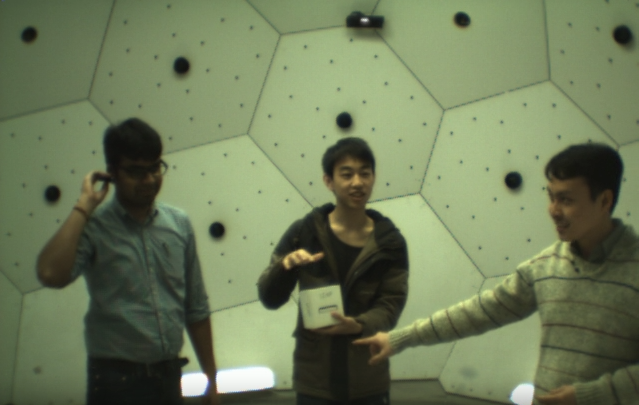
\includegraphics[width=\linewidth]{figures/examples/example1.png}
    \end{subfigure}
    \begin{subfigure}[t]{0.19\linewidth}
      \centering
      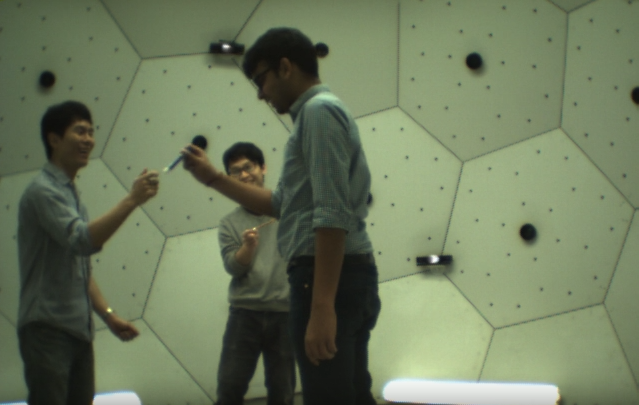
\includegraphics[width=\linewidth]{figures/examples/example2.png}
    \end{subfigure}
    \begin{subfigure}[t]{0.19\linewidth}
      \centering
      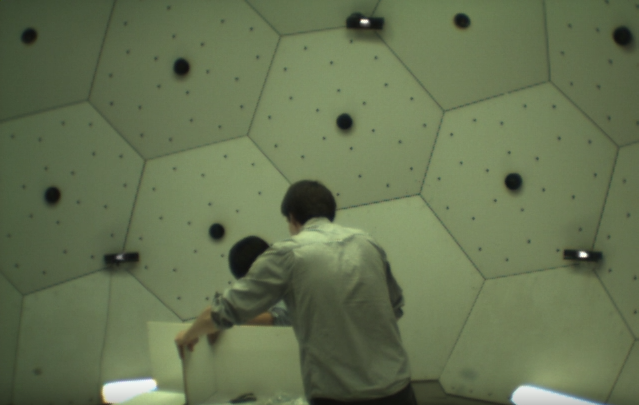
\includegraphics[width=\linewidth]{figures/examples/example3.png}
    \end{subfigure}
    \begin{subfigure}[t]{0.19\linewidth}
      \centering
      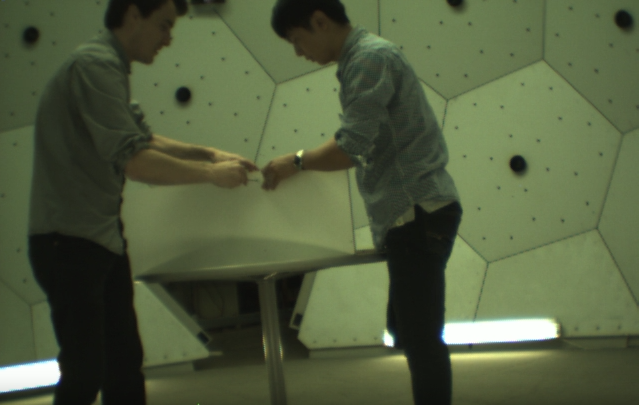
\includegraphics[width=\linewidth]{figures/examples/example4.png}
    \end{subfigure}
    \begin{subfigure}[t]{0.19\linewidth}
      \centering
      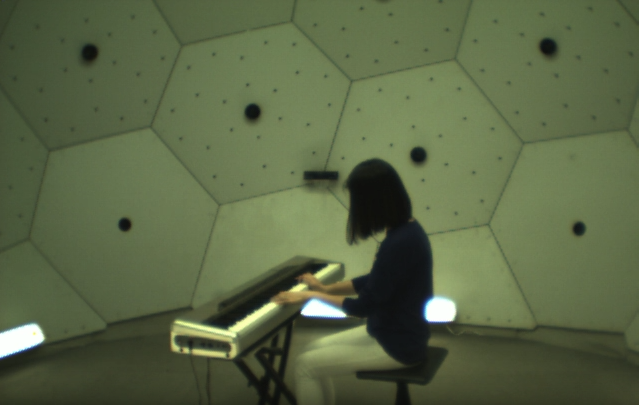
\includegraphics[width=\linewidth]{figures/examples/example5.png}
    \end{subfigure}
  \end{subfigure}
  \begin{subfigure}[t]{\textwidth}
    \begin{subfigure}[t]{0.19\linewidth}
      \centering
      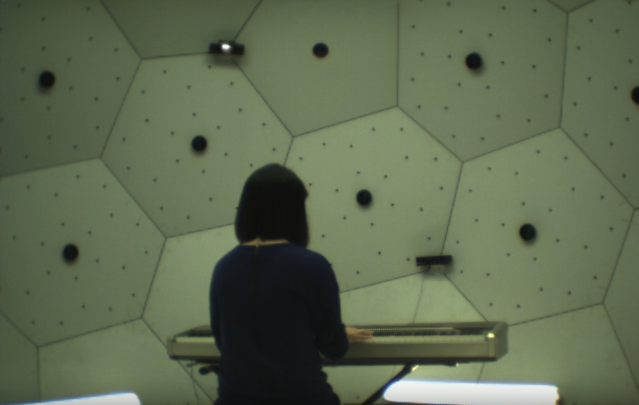
\includegraphics[width=\linewidth]{figures/examples/example6.png}
    \end{subfigure}
    \begin{subfigure}[t]{0.19\linewidth}
      \centering
      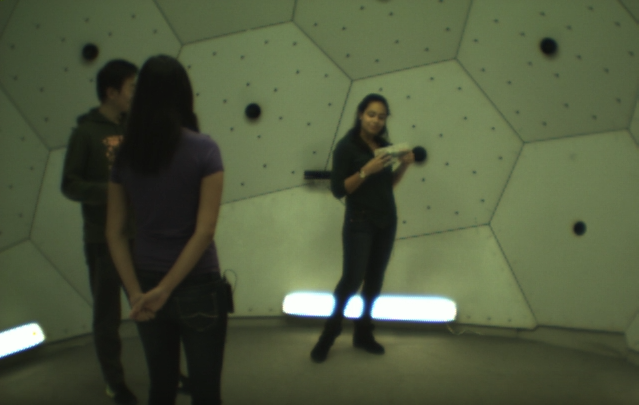
\includegraphics[width=\linewidth]{figures/examples/example7.png}
    \end{subfigure}
    \begin{subfigure}[t]{0.19\linewidth}
      \centering
      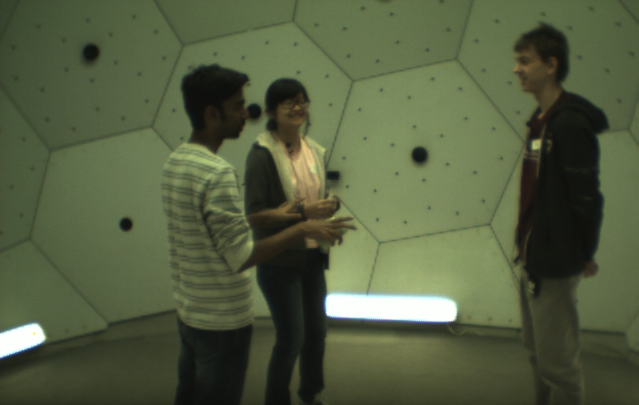
\includegraphics[width=\linewidth]{figures/examples/example8.png}
    \end{subfigure}
    \begin{subfigure}[t]{0.19\linewidth}
      \centering
      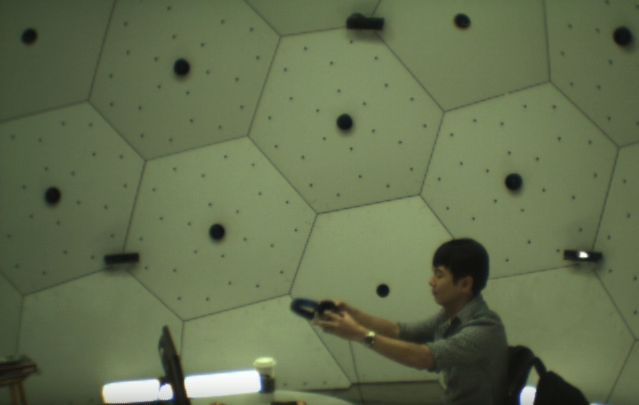
\includegraphics[width=\linewidth]{figures/examples/example9.png}
    \end{subfigure}
    \begin{subfigure}[t]{0.19\linewidth}
      \centering
      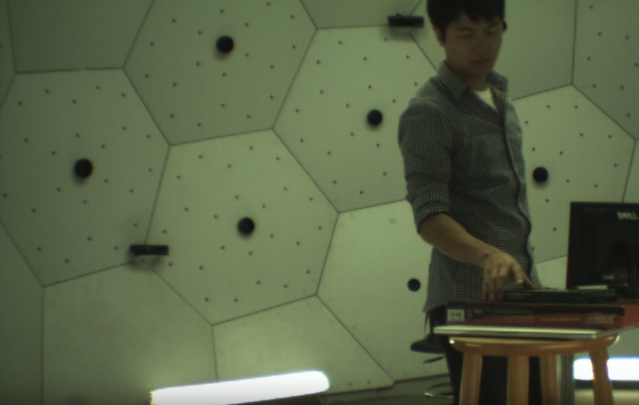
\includegraphics[width=\linewidth]{figures/examples/example10.png}
    \end{subfigure}
  \end{subfigure}
  \caption{A series of example images extracted from the video sequences of the CMU Panoptic dataset.}
  \label{fig:examples}
\end{figure*}

\section{Experimental Evaluation} \label{experiments}

This section of the report will focus on how the proposed system has been experimentally evaluated. Further it covers the dataset used for the experiments and the selected evaluation metrics.


\subsection{Dataset Description} \label{dataset-desc}

For the development and evaluation of the tracking system in this project, the CMU Panoptic Dataset \parencite{Joo_2015_ICCV,Joo_2017_TPAMI,Simon_2017_CVPR} has been used. This is a large-scale dataset that was originally recorded to facilitate research in multi-view social motion capture. \Cref{fig:examples} shows a sample of some still images extracted from the video sequences contained in this dataset.

The complete dataset includes 84 video sequences totaling approximately 11.5 hours of video captured in a specialized 5.49m diameter dome-shaped room equipped with inward facing cameras attached to the outside panels. In total, the recording hardware consists of 511 calibrated cameras, 480 VGA cameras recording at a $640 \times 480$ resolution at 25 fps and 31 HD cameras recording at a $1920 \times 1080$ resolution at 30 fps. The room also contains 10 Kinect II \parencite{kurillo2022evaluating} sensors and 5 DLP projectors. Because of the geometry of the room and the placement of cameras, no single camera is able to view the complete space. This means that while each point in the space is visible from multiple cameras, each camera only captures a partial view of the environment, introducing occlusion and field-of-view limits related challenges for the tracking task.

Crucially, the dataset also includes ground truth 3D skeletons and tracks that were generated by the CMU researchers using algorithms that leverage the entirety of the camera array \parencite{Joo_2015_ICCV}. Ground truth annotations of the dataset are provided in the COCO19 format. To align them with the outputs of the YOLO-based pose estimation networks used in this project \parencite{ultralyticsYOLO}, the ground truth data was pre-processes by converting it into the COCO17 format \parencite{lin2014microsoft}. This was achieved by discarding the two extra joint positions. The dataset also includes the calibration parameters for all available camera views, including camera extrinsics, intrinsics, and distortion parameters.

% TODO change the list of sequences that have been used for testing
Due to computational and time constraints, running the tracking system across all the sequences for the dataset was not reasonable. For this reason, a subset of the dataset was selected for use as the testing set. These sequences where also excluded from the training of the system components as explained in \cref{arch-learning}. The following eight sequences were reserved for testing: \inlinecode{160224_haggling1}, \inlinecode{160906_ian1}, \inlinecode{160906_pizza1}, \inlinecode{161029_build1}, \inlinecode{161029_sports1}, \inlinecode{170221_haggling_m3}, \inlinecode{170915_office1}, and \inlinecode{171026_pose3}. These sequences have been selected to cover a wide verity of different and challenging scenarios. Furthermore, evaluation was performed using only a subset of all camera views. A maximum of 16 VGA-type cameras were utilized per video sequence. These 16 cameras were selected based on the official dataset download script \footnote{\url{https://github.com/CMU-Perceptual-Computing-Lab/panoptic-toolbox/blob/master/scripts/getData.sh}}, which ensures they are approximately uniformly distributed around the dome to provide maximum spatial coverage with a minimal camera count.

In addition to the CMU Panoptic dataset, for some qualitative analysis and demos also the SALSA dataset \parencite{alameda2015salsa} has been used. This dataset represents a much more difficult scenario for the system, however, because it does not contain any ground truth pose annotations, it could not be used for the quantitative evaluations.

\begin{table*}[!ht]
  \centering
  \begin{tabular}{|r|r|c|c|c|c|c|c|c|}
  \hline
    Model & \# Cameras & Detection & Matching & EKF Update & EKF Prediction & Total \\ \hline
    \multirow{4}{*}{YOLO26n-pose}  & 4 & 0.0411 & 0.0131 & 0.0069 & 0.0005 & 0.0616 \\ \cline{2-7}
      & 8 & 0.0850 & 0.0236 & 0.0102 & 0.0007 & 0.1195 \\ \cline{2-7}
      & 12 & 0.1403 & 0.0280 & 0.0118 & 0.0008 & 0.1809 \\ \cline{2-7}
      & 16 & 0.1922 & 0.0355  & 0.0163 & 0.0008 & 0.2448 \\ \hline \hline
    YOLO26s-pose & 4 & 0.1137 & 0.0139 & 0.0083 & 0.0007 & 0.1365 \\ \hline
    YOLO26m-pose & 4 & 0.2866 & 0.0140 & 0.0087 & 0.0007 & 0.3100 \\ \hline
    YOLO26l-pose & 4 & 0.3408 & 0.0143 & 0.0090 & 0.0007 & 0.3648 \\ \hline
  \end{tabular}
  \caption{Average per-frame runtime of the tracking system for different camera and model configurations. Times are given in seconds.}
  \label{fig:perf}
\end{table*}

\begin{table*}[!ht]
  \centering
  \begin{tabular}{|r|r|c|c|c|c|c|}
  \hline
    Model & \# Cameras & MOTA & MOTP & MPJPE & Precision & Recall \\ \hline \hline
    \multirow{4}{*}{YOLO26n-pose} & 4 & 0.781 & 5.488 & 8.250 & 0.890 & 0.890 \\ \cline{2-7}
      & 8 & 0.924 & 3.235 & 3.341 & \textbf{0.939} & 0.994 \\ \cline{2-7}
      & 12 & \textbf{0.926} & 3.066 & 3.146 & 0.939 & 0.996 \\ \cline{2-7}
      & 16 & 0.920 & \textbf{2.749} & \textbf{2.834} & 0.934 & \textbf{0.996} \\ \hline \hline
    YOLO26s-pose & 4 & 0.785 & 5.151 & 8.616 & 0.888 & 0.899 \\ \hline
    YOLO26m-pose & 4 & 0.807 & 4.976 & 7.466 & 0.897 & 0.913 \\ \hline
    YOLO26l-pose & 4 & 0.809 & 4.792 & 7.674 & 0.898 & 0.915 \\ \hline
  \end{tabular}
  \caption{Evaluation results for the baseline configuration with different camera and model configurations. MOTA, MOTP, Precision, and Recall have been computed with an average of 15 centimeters Euclidean distance as the matching threshold. MOTP and MPJPE are given as mean per-joint Euclidean distance in centimeters. The best result in each column is highlighted in bold.}
  \label{fig:eval-results}
\end{table*}


\subsection{Evaluation Procedure} \label{eval-proc}

For this project the system has been evaluated by comparing its 3D tracking predictions frame-by-frame against the ground truth annotations in the CMU Panoptic dataset. The experiments were run across all eight selected sequences mentioned in \cref{dataset-desc}, evaluating various combinations of YOLO pose estimation models, testing \inlinecode{YOLO26n-pose}, \inlinecode{YOLO26s-pose}, \inlinecode{YOLO26m-pose}, and \inlinecode{YOLO26l-pose}, spacial view densities of 4, 8, 12, and 16, as well as testing different configurations of the system, such as with or without skeletal constraints. Note only the \inlinecode{YOLO26n-pose} model has been tested with more than 4 cameras and that the more advanced configurations of the system have also only been tested in the 4 camera setting. All evaluations were performed on AMD Ryzen AI 9 HX 370 CPU with most PyTorch \parencite{paszke2019pytorch,ansel2024pytorch} operation running on the integrated AMD Radeon 890M GPU.

For the baseline system configuration, parameters of the system were initialized heuristically rather than via exhaustive grid-search or end-to-end learning. While these rigid parameter values are functional, the system performs better when using the components that were learned from data as shown in \cref{results}.

For the baseline system, detection thresholds for the YOLO based detector we set to $\tau_{obj} = 0.5$ and $\tau_{kpt} = 0.25$, using also $N_{kpt} = 3$ as the minimum number of visible keypoints. The minimum pixel variance has been set to $\sigma_{min}^2 = 16.0$ pixels$^2$, with visibility and invisibility scale variances set to $\sigma_{vis}^2 = 0.005$ and $\sigma_{inv}^2 = 5$. The matching thresholds for both cross-view and prediction-view matching have both been set to $\theta_{mn} = \theta_{mo} = 0$. For the tracking lifecycle we configured the age for tentative track promotion to $N_{age} = 3$ and the maximum duration without detections for active tracks to $N_{inv} = 10$. Finally, the continuous physic matrices have been set as follows:
\begin{align*}
    \mathbf{F} = \begin{bmatrix} \mathbf{0}_{51 \times 51} & \mathbf{I}_{51 \times 51} \\ \mathbf{0}_{51 \times 51} & -0.2 \cdot \mathbf{I}_{51 \times 51} \end{bmatrix}, & \;
    \mathbf{Q} = \begin{bmatrix} \sigma_{p}^2 \cdot \mathbf{I}_{51 \times 51} & \mathbf{0}_{51 \times 51} \\ \mathbf{0}_{51 \times 51} & \sigma_{v}^2 \cdot \mathbf{I}_{51 \times 51} \end{bmatrix}
\end{align*}
with $\sigma_{v}^2 = (3 \frac{m}{s})^2$ and $\sigma_{p}^2 = (1 cm)^2$. This matrix models constant velocity dynamics with a damping term of $-0.2$ on velocity to stabilize motion predictions.


\subsection{Evaluation Metrics} \label{eval-metrics}

To measure tracking and reconstruction performance, this project makes use of standard metrics from the Multi-Object Tracking and 3D Pose Estimation literature \parencite{bernardin2008evaluating,ionescu2013human3}. All measures are reported in centimeters, and we use a mean joint error of 15 centimeters as the threshold for matches for all metrics except MPJPE.

\paragraph{Mean Per-Joint Position Error (MPJPE)}
MPJPE measures the average 3D Euclidean distance between predicted and ground truth keypoints across all matched frames and joints.
\begin{align*}
    \text{MPJPE} &= \frac{1}{N_{matched}} \sum_{i=1}^{N_{matched}} \left( \frac{1}{17} \sum_{k=1}^{17} \|\mathbf{p}_{k,i}^{pred} - \mathbf{p}_{k,i}^{gt}\|_2 \right)
\end{align*}
For this metric we do not apply a matching threshold, instead matching all predictions against the best matching ground truth track via Hungarian method based assignment.

\paragraph{Multi-Object Tracking Accuracy (MOTA)}
MOTA evaluates overall tracking performance by accounting for three types of errors, false positives, false negatives, and identity switches:
\begin{align*}
    \text{MOTA} &= 1.0 - \frac{\sum_{t} \text{FN}_t + \text{FP}_t + \text{IDS}_t}{\sum_{t} \text{GT}_t}
\end{align*}
where $\text{FN}_t$ is the number of false negatives, $\text{FP}_t$ the number of false positives, $\text{IDS}_t$ that of identity switches, and $\text{GT}_t$ is the number of ground truth individuals in frame $t$.

\paragraph{Multi-Object Tracking Precision (MOTP)}
MOTP measures the alignment of tracked objects by calculating the average distance error for correctly matched targets. Note that in contrast to MPJPE this metric is only computed over the true positives matched within the 15 centimeters maximum threshold.
\begin{align*}
    \text{MOTP} &= \frac{\sum_{t,d} \frac{1}{17} \sum_{k=1}^{17} \|\mathbf{p}_{t,d,k}^{pred} - \mathbf{p}_{t,d,k}^{gt}\|_2}{\sum_{t} \text{TP}_t}
\end{align*}
where $\text{TP}_t$ is the number of true positives.

\paragraph{Precision and Recall}
Finally, we also report the standard precision and recall metrics.
\begin{align*}
    \text{Precision} = \frac{\sum_t \text{TP}_t}{\sum_t \text{TP}_t + \text{FP}_t}, &\quad \text{Recall} = \frac{\sum_t \text{TP}_t}{\sum_t \text{TP}_t + \text{FN}_t}
\end{align*}



\section{Results and Discussion} \label{results}

This section of the report will present the evaluation results obtained by the developed system on the chosen dataset. It further contains also discussion of the presented results and possible reasons for the observed deficiencies.

\subsection{Runtime Efficiency} \label{effic}

% TODO mention that efficiency has been tested using the simple version without learned component ot skeletal constraints 
% TODO update all of the results
\begin{table*}[!ht]
  \centering
  \begin{tabular}{|r|r|c|c|c|c|c|c|c|}
  \hline
    Model & \# Cameras & Detection & Matching & EKF Update & EKF Prediction & Total \\ \hline
    \multirow{4}{*}{YOLO26n-pose}  & 4 & 0.0411 & 0.0131 & 0.0069 & 0.0005 & 0.0616 \\ \cline{2-7}
      & 8 & 0.0850 & 0.0236 & 0.0102 & 0.0007 & 0.1195 \\ \cline{2-7}
      & 12 & 0.1403 & 0.0280 & 0.0118 & 0.0008 & 0.1809 \\ \cline{2-7}
      & 16 & 0.1922 & 0.0355  & 0.0163 & 0.0008 & 0.2448 \\ \hline \hline
    YOLO26s-pose & 4 & 0.1137 & 0.0139 & 0.0083 & 0.0007 & 0.1365 \\ \hline
    YOLO26m-pose & 4 & 0.2866 & 0.0140 & 0.0087 & 0.0007 & 0.3100 \\ \hline
    YOLO26l-pose & 4 & 0.3408 & 0.0143 & 0.0090 & 0.0007 & 0.3648 \\ \hline
  \end{tabular}
  \caption{Average per-frame runtime of the tracking system for different camera and model configurations. Times are given in seconds.}
  \label{fig:perf}
\end{table*}

\Cref{fig:perf} shows the mean per-frame runtime of the developed tracking system across the selected test sequences for different camera count and model capacity configurations. It can be seen that across every single configuration, the detection step consumes the vast majority of the processing time. For the base setup with YOLO26n-pose and 4 camera vies, detection takes 0.0445 seconds out of a 0.0697-second total which equals approximately 64\% of the frame time. This discrepancy becomes wider when increasing the model capacity. For the larges model, YOLO26l-pose, still with only 4 cameras, the detection takes up to 0.2613 seconds out of a total of 0.2879 seconds, which represents approximately 91\% of the time.

When adding more camera views to the system using the smallest model, the computational load predictably increases. Because the detection model has to run a forward pass on every single camera feed, detection time scales almost perfectly linearly with the number of cameras, from 0.045s for 4 cameras to 0.181s for 16. Steps like matching and EKF updates also scale up as camera counts increase because these need to handle more cross-camera data points to associate and filter. However, their growth is somewhat slower than the linear increase for detection. The EKF prediction step is largely a negligible part of the overall system runtime.

When keeping the camera count at 4 but upgrading the YOLO architecture to larger capacity version, it can be observed that the cost increases significantly. Upgrading from YOLO26n-pose to YOLO26s-pose doubles the detection time, going from 0.0445s to 0.0876s. However, jumping to the medium or large version causes a massive spike, tripling the time to over a quarter of a second. Predictably, only the runtime for the detection step is affected by increasing the model capacity and matching, EKF update, and Prediction remain almost entirely unchanged across all four model variants.

With the fastest configuration tested, the system achieves only around 14.3 fps. This is likely insufficient for real-time applications. However, it should be noted that not much effort has gone into optimization of the implementation, and that the test where performed on relatively weak integrated GPU hardware.

% TODO mention that these results for camera count, scene difficulty, and model size were using the simple configuration.
% TODO update all of the results
\begin{table*}[!ht]
  \centering
  \begin{tabular}{|r|r|c|c|c|c|c|}
  \hline
    Model & \# Cameras & MOTA & MOTP & MPJPE & Precision & Recall \\ \hline \hline
    \multirow{4}{*}{YOLO26n-pose} & 4 & 0.781 & 5.488 & 8.250 & 0.890 & 0.890 \\ \cline{2-7}
      & 8 & 0.924 & 3.235 & 3.341 & 0.939 & 0.994 \\ \cline{2-7}
      & 12 & \textbf{0.926} & 3.066 & 3.146 & \textbf{0.939} & 0.996 \\ \cline{2-7}
      & 16 & 0.920 & \textbf{2.749} & \textbf{2.834} & 0.934 & \textbf{0.996} \\ \hline \hline
    YOLO26s-pose & 4 & 0.785 & 5.151 & 8.616 & 0.888 & 0.899 \\ \hline
    YOLO26m-pose & 4 & 0.807 & 4.976 & 7.466 & 0.897 & 0.913 \\ \hline
    YOLO26l-pose & 4 & 0.809 & 4.792 & 7.674 & 0.898 & 0.915 \\ \hline
  \end{tabular}
  \caption{Evaluation results for different camera and model configurations. MOTA, MOTP, Precision, and Recall have been computed with an average of 15 centimeters Euclidean distance as the matching threshold. MOTP and MPJPE are given as mean per-joint Euclidean distance in centimeters. The best result in each column is highlighted in bold.}
  \label{fig:eval-results}
\end{table*}

% TODO update with correct scenes
% TODO update all of the results
\begin{table*}[!ht]
  \centering
  \begin{tabular}{|r|c|c|c|c|c|}
  \hline
    Scene & MOTA & MOTP & MPJPE & Precision & Recall \\ \hline \hline
    \inlinecode{160224_haggling1} & 0.861 & 3.974 & 4.961 & 0.900 & 0.971 \\ \hline
    \inlinecode{160906_ian1} & 0.607 & 4.758 & 9.149 & 0.779 & 0.839 \\ \hline
    \inlinecode{160906_pizza1} & 0.823 & 5.595 & 8.112 & 0.909 & 0.915 \\ \hline
    \inlinecode{161029_build1} & 0.950 & 4.070 & 4.363 & 0.976 & 0.974 \\ \hline
    \inlinecode{161029_sports1} & 0.631 & 4.291 & 9.278 & 0.783 & 0.869 \\ \hline
    \inlinecode{170221_haggling_m3} & 0.943 & 3.869 & 4.198 & 0.960 & 0.984 \\ \hline
    \inlinecode{170915_office1} & 0.994 & 4.114 & 4.136 & 0.997 & 0.998 \\ \hline
    \inlinecode{171026_pose3} & 0.993 & 2.993 & 3.035 & 0.995 & 0.997 \\ \hline
  \end{tabular}
  \caption{Evaluation results for different scenes averaged over all performed evaluations. Evaluation metrics have been calculates as described in \cref{fig:eval-results}.}
  \label{fig:eval-by-scene}
\end{table*}

% TODO add result of the impact of the skeletal constraints and the learned components.
\begin{table*}[!ht]
  \centering
  \begin{tabular}{|r|c|c|c|c|c|}
  \hline
    Configuration & MOTA & MOTP & MPJPE & Precision & Recall \\ \hline \hline
    Baseline & 0.781 & 5.488 & 8.250 & 0.890 & 0.890 \\ \hline
    Constraints & 0.842 & 5.139 & 7.264 & 0.920 & 0.923 \\ \hline
    Learned Kalman & 0.880 & 4.679 & 5.801 & 0.937 & 0.944 \\ \hline
    Custom YOLO & 0.886 & \textbf{3.788} & 5.318 & 0.941 & 0.946 \\ \hline
    LK + CY & 0.893 & 4.083 & 5.184 & 0.944 & \textbf{0.950} \\ \hline
    Tuned & \textbf{0.897} & 3.840 & \textbf{4.917} & \textbf{0.948} & 0.949 \\ \hline
  \end{tabular}
  \caption{Evaluation results for configurations of the system. All values are given for a setup with four cameras and the YOLO26n-pose model. Evaluation metrics have been calculates as described in \cref{fig:eval-results}. The best result in each column is highlighted in bold.}
  \label{fig:eval-by-config}
\end{table*}

\begin{figure*}[ht!]
  \centering
  \hfill
  \begin{subfigure}[t]{0.19\linewidth}
    \centering
    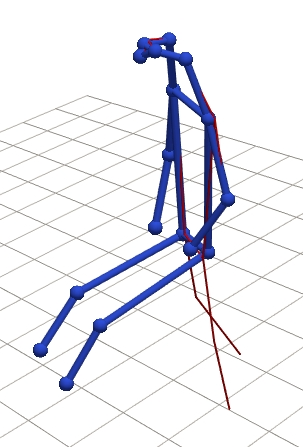
\includegraphics[width=\linewidth]{figures/qualitative1.png}
    \caption{Partially occluded person.}
    \label{fig:qual-occlusion}
  \end{subfigure}
  \hfill
  \begin{subfigure}[t]{0.19\linewidth}
    \centering
    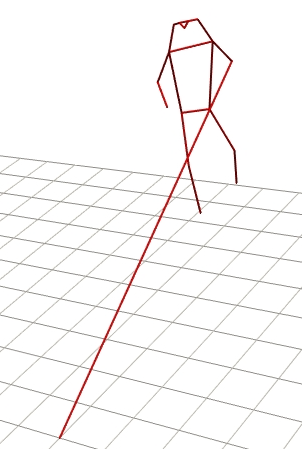
\includegraphics[width=\linewidth]{figures/qualitative2.png}
    \caption{Inactive track seen by only one camera.}
    \label{fig:qual-single}
  \end{subfigure}
  \hfill
  \begin{subfigure}[t]{0.19\linewidth}
    \centering
    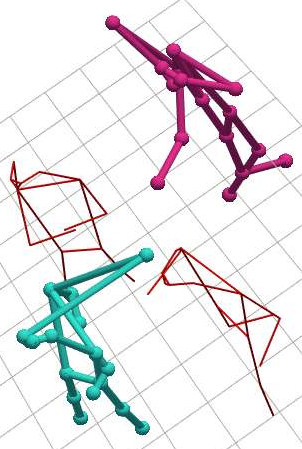
\includegraphics[width=\linewidth]{figures/qualitative3.png}
    \caption{Active track seen by only one camera.}
    \label{fig:qual-single2}
  \end{subfigure}
  \hfill
  \begin{subfigure}[t]{0.19\linewidth}
    \centering
    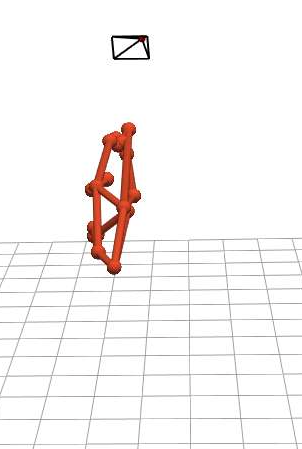
\includegraphics[width=\linewidth]{figures/qualitative4.png}
    \caption{Detection of person while exiting.}
    \label{fig:qual-leave}
  \end{subfigure}
  \hfill
  \caption{Some qualitative samples extracted from the evaluation results on the test set that exhibit commonly seen issues with the tracking system. Ground truth skeletons are drawn using thing red lines, while predicted skeletons are drawn thicker and with different colors per track.}
  \label{fig:qual}
\end{figure*}

\subsection{Quantitative Results} \label{quant}

Quantitative results for the system on the chosen test sequences can be found in \cref{fig:eval-results}. When keeping the model fixed to YOLO26n-pose and increasing the number of cameras from 4 to 16, a significant reduction in pose and localization errors can be observed. The joint position error decreases drastically by about half, from 5.439 cm down to 2.576 cm. This indicates that incorporating more viewpoints substantially improves 3D localization and pose estimation accuracy. Also, the increase in camera views brings improvements in recall. Recall increases from 0.975 with 4 cameras to 0.998 when using 16 cameras, indicating fewer missed detections likely because the cameras now cover more angles that would otherwise not be visible. There exists a slight trade-off in tracking accuracy and precision. Adding more cameras leads to a decrease in precision from 0.966 for 4 cameras to 0.955 with 16. This can be explained by the fact that more camera views introduce a higher likelihood of false positives and could also indicate limitations in the association algorithm. MOTA hits a sweet spot of 0.960 with 8 cameras. 

In contrast, when keeping the camera count fixed at 4 and scaling up the model complexity from YOLO26n-pose to YOLO26l-pose, we see improvements in all metrics. The largest model achieves the best overall MOTA of 0.960 and precision of 0.977. Upgrading the model capacity also reduces MPJPE from 5.439 cm to 4.554 cm. However, the improvement in this metric is not as significant as with the addition of more cameras.

Finally, \cref{fig:eval-by-scene} shows the average performance per scene across performed evaluations. It can be seen that the \inlinecode{160224_haggling1} scene is the one with the lowest performance metrics. In this scene, MOTA and Precision suffer from a large increase in false positives. This scene contains the most entries and exists from the room as well as more close contact, which the tracking algorithm can struggle with. The system performs particularly well on \inlinecode{161029_piano4} and \inlinecode{170915_office1}. This is largely because in these scenes the persons are in the room for the entire duration of the video sequence, avoiding a big source of errors for the system.


\subsection{Qualitative Results} \label{qual}

Some qualitative evaluation has also been performed for this project.

\subsubsection{Impact of the Skeletal Constraints}

% TODO add another figure with SALSA
% TODO add another figure with Covision data
% TODO talk about impact of the skeletal constraints

\subsubsection{Common Failure Modes}

% TODO mention that some if the failure modes are solved by the skeletal constraints
The results of the system on the tests sequences has been visualized and a number of common issues have been identified. Some examples of these failure modes are shown in \cref{fig:qual}.

\paragraph{Partially Occluded Person}
One very common failure mode is depicted in \cref{fig:qual-occlusion}. When a person is partially occluded in all camera views, then the position of the unobserved keypoints tends to shift in unnatural ways, as can be seen with the legs keypoints in the given example. This problem is made worse by the fact that the YOLO model tend to predict invisible keypoints in unnatural positions, and while their visibility score is low, it can still commutatively have a significant effect over multiple frames. This issue causes increased joint position errors.

\paragraph{Inactive Track Seen by Only One Camera}
Another commonly observed failure is shown in \cref{fig:qual-single}. When a person first enters the room, typically only one camera can see them. This means that it is not possible to create a new track for that person. This causes false positives, and therefore reduced MOTA and Recall, whenever a person enters the room.

% TODO mention that this is less of a problem with the skeletal constraints
\paragraph{Active Track Seen by Only One Camera}
\Cref{fig:qual-single2} shows another issue that can occur when only a single camera is able to see a given person. In this case, the track has already been initialized, but the person has moved into a location where they are no longer seen by two cameras. In this case the depth coordinate from the camera can drift as the person moves, causing distorted skeletons before and behind the actual ground truth.

\paragraph{Detection of Person While Exiting}
\Cref{fig:qual-leave} show a failure that occurs when a person leaves the room. In this case, the camera that is pointing at the exit will see the person for longer than the actual ground truth indicates. This causes false positives and therefore worse MOTA and Precision. Note that in this case we also have the above mention issue of an active track seen by only one camera.



\section{Conclusion and Outlook} \label{conclusion}

In conclusion, in this project a complete end-to-end 3D multi-person tracking pipeline was designed, implemented, and evaluated.
The quantitative evaluation on the CMU Panoptic dataset provided some architectural insight. Spatial viewpoint density exhibits a far higher return on tracking accuracy than increasing deep learning model capacity. Scaling the camera view count from 4 to 16 with the YOLO26n-pose model reduced the mean per-joint position error from 8.25 cm down to 2.83 cm. In contrast, replacing this lightweight model with the heavy YOLO26l-pose model under a fixed 4-camera setup yielded smaller accuracy gains at the cost of a massive computational bottleneck, dropping system throughput to approximately 3 FPS.
Additionally, performance can also be significantly improved with the addition of skeletal constraints as well as the use of learning from data for different components.  

Despite the relatively high localization accuracy of the system under optimal conditions, there remain several limitations. As demonstrated in the qualitative evaluations, tracking quality degrades when targets are partially occluded or not in view of the camera views. Since 3D initialization requires triangulation across at least two views, the system also exhibits tracking delays during entry and spatial drifting during single-camera visibility. Further, the way the system has been adapted to the dataset by training individual components separately limits the amount of adaptation.

Possible future improvements to address these limitations could include fully end-to-end training of the system parameters from the dataset instead of training components separately. A further improvement could be the addition of further anatomical plausibility constraints on the state predictions, such as realistic joint angles. These constraints could possibly be included similar to the existing limb length constraints using a pseudo-measurement. Also, the addition of additional information sources, such as monocular depth values could make it possible to track people even using single camera views. Exploring more advanced filtering methods such as particle filters, potentially also using occlusion aware likelihoods could be promising future directions. Finally, the evaluation in this project has been performed only on the CMU Panoptic dataset. As such, the evaluation of the system using a larger set of more diverse sequences would be highly valuable to uncover further areas for improvement.


\printbibliography

\end{document}
